\documentclass{beamer}
\usepackage[utf8]{inputenc}
\usepackage{graphics}
\usepackage{subcaption}
\mode<presentation> {
\usetheme{unc}}
\setbeamertemplate{navigation symbols}{} % To remove the navigation symbols from the bottom of all slides uncomment this line

\usepackage{graphicx} % Allows including images
\usepackage{booktabs} % Allows the use of \toprule, \midrule and \bottomrule in tables


\usepackage{hyperref}
\hypersetup{linkcolor=blue,colorlinks=true}


% Remove symbols
\beamertemplatenavigationsymbolsempty


%\usetheme{default}

\usefonttheme{serif}

%----------------------------------------------------------------------------------------
%	TITLE PAGE
%----------------------------------------------------------------------------------------


\title[The Three I's]{\LARGE{Interests, Interactions, Institutions and Game Theory}}
\author[POLI 150]{Steven Saroka}
\institute{POLI 150}
\date{18 January 2024}


\begin{document}

\begin{frame}
\titlepage % Print the title page as the first slide
\end{frame}


%\begin{frame}
%\frametitle{Overview} % Table of contents slide, comment this block out to remove it
%\tableofcontents % Throughout your presentation, if you choose to use \section{} and \subsection{} commands, these will automatically be printed on this slide as an overview of your presentation
%\end{frame}


%%% SLIDE TEMPLATES

% Template for images
% \begin{frame}{\LARGE Kurdistan}
%     \centering
% \includegraphics[width=\textwidth,height=0.8\textheight,keepaspectratio]{}
% \end{frame}

% %% Core template for the slides
% \begin{frame} 
% \frametitle{\LARGE{}}
% \end{frame}

%----------------------------------------------------------------------------------------
%	PRESENTATION SLIDES
%----------------------------------------------------------------------------------------


%% Slide outline
\begin{frame} 
	\frametitle{\LARGE{Today's Class}}
	\begin{itemize}
			\item Interests, Interactions, Institutions
			\\~\\ 
			\item Strategic Interaction 
			\\~\\
			\item Game Theory Primer
	\end{itemize}
\end{frame}

\begin{frame} 
	\frametitle{\LARGE{Central Question}}
	\begin{center}
	    	\LARGE How do we theorize and explain world politics? 
   	\end{center}
\end{frame}

\begin{frame} 
	\frametitle{\LARGE{Key terms}}
	\begin{itemize}
		\item Interests
		\item Strategic Interactions
		\item Institutions
		\item Rationality
		\item Cooperation
		\item Bargaining
		\item Prisoner's Dilemma
		\item Collective Action Problem
	\end{itemize}
\end{frame}

\begin{frame} 
	\frametitle{\LARGE{General Goal: Theory Development}}
	\begin{itemize}
		\item Political scientists develop \textbf{theories}: a logically consistent set of statements that explain a phenomenon of interest. \pause
		\item \textbf{Good theories simplify complexity} to identify the most important factors in explaining that phenomenon. \pause
		\item Goal is \textbf{probabilistic claims}: successful theories identify the factors that make something more or less likely. 
		\begin{itemize}
			\item Political scientists tend to avoid absolute claims, unlike theories from the physical sciences.
		\end{itemize}	
	\end{itemize}
\end{frame}

\begin{frame} 
	\frametitle{\LARGE{Theory Components}}
	\begin{itemize}
		\item \textbf{Actors}: the basic units of any analysis.  \pause
		\item What is the primary actor in IR? \pause
		\begin{itemize}
			\item The state.
		\end{itemize}
		\item All actors have \textbf{interests}: the political goals and objectives they pursue; what they want to achieve in any given situation.
	\end{itemize}
\end{frame}

\begin{frame} 
	\frametitle{\LARGE{Interest Examples}}
	\centering
	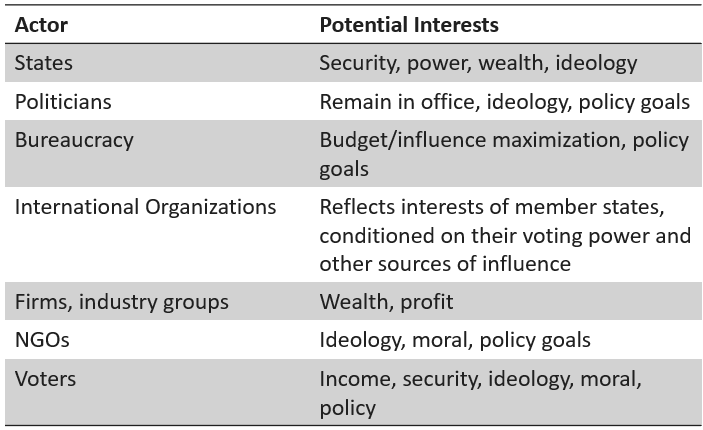
\includegraphics[width=\textwidth,height=0.8\textheight,keepaspectratio]{interests.png}
\end{frame}

\begin{frame} 
	\frametitle{\LARGE{Interactions}}
	\begin{itemize}
		\item Actors are not alone - their actions impact each other.
		\item \textbf{Interactions}: how the choices of two or more actors combine, producing political outcomes. \pause
		\item These interactions can be \textbf{strategic}: each actor's strategy depends on what they anticipate other actors will do. \pause
		\item Actors purposefully develop strategies that they believe will be the best response to the anticipated strategies of others. 
		\item We'll come back to this shortly with game theory.
	\end{itemize}
\end{frame}

\begin{frame} 
	\frametitle{\LARGE{Institutions}}
	\begin{itemize}
		\item \textbf{Institutions}: a common set of rules shared amongst actors that structure interactions in specific ways. \pause
		\item Examples? \pause
		\begin{itemize}
			\item UN
			\item NATO
			\item World Trade Organization
			\item International Monetary Fund
		\end{itemize}
	\end{itemize}
\end{frame}
	
\begin{frame} 
	\frametitle{\LARGE{Applying the Framework}}
	\begin{itemize}
		\item Identify the relevant actors and their interests \pause
		\\~\\ 
		\item Describe the choices or actions they must choose from \pause 
		\\~\\ 
		\item Think about how those choices interact to produce outcomes \pause 
		\\~\\ 
		\item Consider whether institutions structure the interaction
	\end{itemize}
\end{frame}

\begin{frame} 
	\frametitle{\LARGE{The Iraq War}}
	\centering
	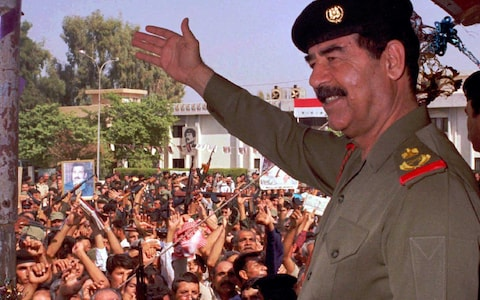
\includegraphics[width=\textwidth,height=0.8\textheight,keepaspectratio]{Hussein.jpg}
\end{frame}

\begin{frame} 
	\frametitle{\LARGE{Building up to the Iraq War}}
	\begin{itemize}
		\item Gulf War in 1991
		\item US- and UN-led sanctions throughout 1990s
		\item 9/11 and the War on Terror
		\item George W. Bush argues that Iraq has WMDs; does not get UN support for intervention
		\item March 2003: US invades Iraq with intent to overthrow the regime
	\end{itemize}
\end{frame}

\begin{frame} 
	\frametitle{\LARGE{The Iraq War}}
	\centering
	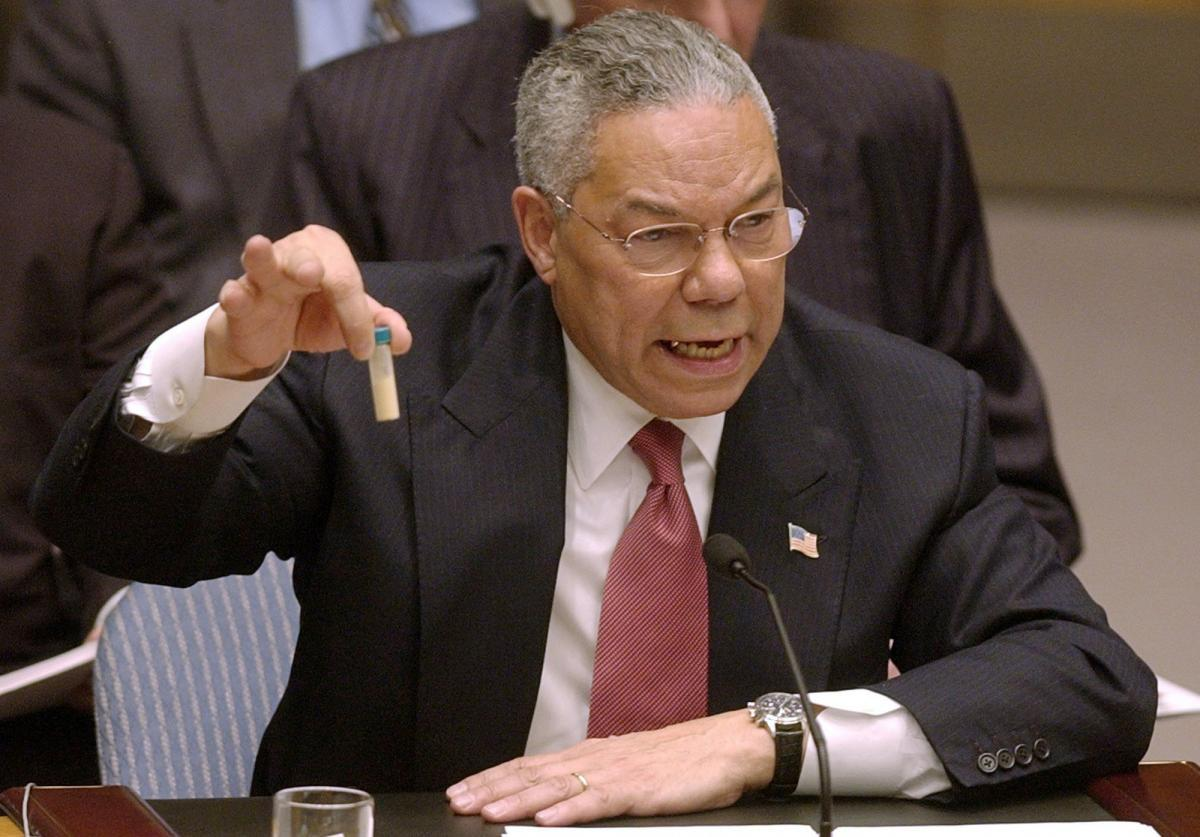
\includegraphics[width=\textwidth,height=0.8\textheight,keepaspectratio]{Powell.jpg}
\end{frame}


\begin{frame} 
	\frametitle{\LARGE{The Iraq War and its effects}}
	\begin{itemize}
		\item May 2003: Bush declares ``mission accomplished"
		\item Insurgency continues throughout the 2000s
		\item January 2007: Bush pledges surge of troops to Iraq
		\item December 2011: Obama withdraws
		\item June 2014: Obama dispatches troops to respond to Islamic State 
		\item December 2021: Roughly 2,500 US troops in Iraq in support roles
	\end{itemize}
\end{frame}

\begin{frame} 
	\frametitle{\LARGE{Casualties as of November 2019}}
	\href{https://watson.brown.edu/costsofwar/}{Costs of War Project}
	\begin{itemize}
		\item 4,572 US troops, 3,588 US contractors, est. 50,000 Iraqi military and police deaths
		\item Est. 37,000 opposition fighter deaths
		\item Est. 200,000 civilian deaths
		\item Economic cost: Nearly \$2 trillion for the US alone
	\end{itemize}
\end{frame}

\begin{frame} 
	\frametitle{\LARGE{Group Discussions}}
	\begin{itemize}
		\item Who are the relevant actors?
		\\~\\
		\item What are the actions they could have taken? 
		\\~\\ 
		\item How did the actions that they chose interact to produce outcomes? 
		\\~\\ 
		\item (How) did institutions structure the interaction? 
	\end{itemize}
\end{frame}
	
\begin{frame} 
	\frametitle{\LARGE{Institutions and Anarchy}}	
	\begin{itemize}
		\item But what about anarchy? \pause
		\item Most states follow institutional rules most of the time. Why? \pause
		\item Answering this requires answering a bigger question...
	\end{itemize}
\end{frame}

\begin{frame} 
	\frametitle{\LARGE{Interaction Types}}
	\centering
\LARGE{What kind of interactions do we observe between actors?}
\end{frame}

\begin{frame} 
	\frametitle{\LARGE{Strategic Interactions}}
	\begin{itemize}
		\item Almost all of the interactions we discuss in this course are \textbf{strategic interactions}: Each actor’s strategy depends on what strategy they anticipate other actors will use. \pause
		\item Phrased differently, what one actor expects others to do shapes their own decision. \pause
		\item Strategic interactions usually take place under \textbf{incomplete information}: any given actor does not know for certain what other actors will do or want. \pause
		\item Thus, strategic interactions involve attempts by actors to successfully anticipate the actions of others.  \pause
		\item This gives rise to two fundamental different types of strategic interaction: \textbf{cooperation} and \textbf{bargaining}.
	\end{itemize}
\end{frame}


 \begin{frame} 
 \frametitle{\LARGE{Game Theory}}
    \begin{itemize}
         \item We can analyze these strategic interactions through \textbf{game theory}: A mathematical way to model what two or more actors (people, states, groups, etc.) do when acting strategically. \pause  
         \item Game theory allows us to find stable outcomes that result from strategic interaction. \pause 
         \item Game theory assumes that all actors are \textbf{rational}.
     \end{itemize}
 \end{frame}

\begin{frame} 
	\frametitle{\LARGE{Game Theory: Rational Actors}}
	\begin{itemize}
		\item A rational actor, by definition, has \textbf{complete}, \textbf{ordered}, and \textbf{transitive} interests (also called ``preferences"). \pause 
		\begin{itemize}
			\item Complete: the actor has some kind of preference for all possible outcomes of a situation. \pause
			\item Ordered: we can rank those preferences in some way. \pause
			\item Transitive: if the actor prefers outcome A to B and B to C, they must prefer A to C. \pause 
		\end{itemize}
		\item This assumption is not always descriptively accurate. \pause 
		\item But it is especially suited to studying politics. 
	\end{itemize}
\end{frame}

 \begin{frame} 
	\frametitle{\LARGE{Game Theory}}
	\begin{itemize}
		\item Game theory lets us analyze both cooperation and bargaining. \pause
		\item \textbf{In any game-theoretic analysis, we always assume all the actors are rational.}
		\begin{itemize}
			\item If this assumption does not hold, game theory stops working.
		\end{itemize}
	\end{itemize}
\end{frame}

\begin{frame} 
	\frametitle{\LARGE{Cooperation}}
	\textbf{Cooperation}: an interaction in which two or more actors adopt policies that make at least one actor better off relative to the status quo without making others worse off.
	\begin{itemize}
		\item Also called positive-sum game.
		\item Cooperating actors are often able to reach the \textbf{Pareto Frontier}: The possible divisions of the maximum benefit for all actors.
	\end{itemize}
\end{frame}

\begin{frame} 
	\frametitle{\LARGE{Cooperation}}
	\centering	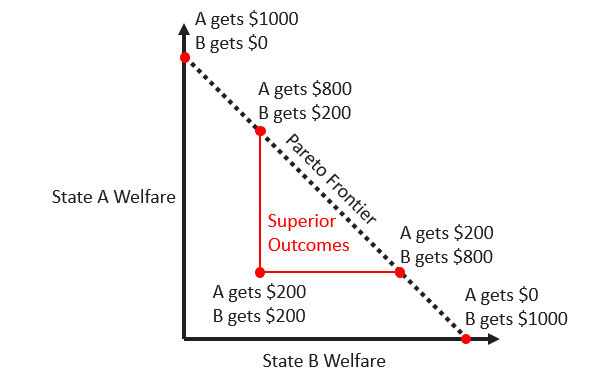
\includegraphics[width=\textwidth,height=0.8\textheight,keepaspectratio]{cooperation.png}
\end{frame}


\begin{frame} 
\frametitle{\LARGE{Cooperation Types - Coordination}}
     \begin{itemize}
         \item \textbf{Coordination:} All actors will benefit from cooperating, and none have incentives to defect. \pause
         \begin{itemize}
         	\item \textbf{Defect}: game theory term for an actor choosing the non-cooperative choice.
             \item In coordination, actors have no incentive to defect. \pause
         \end{itemize}
         \item Example: driving on the same side of the road. \pause
         \begin{itemize}
         	\item Everyone benefits from driving on the same side (fewer crashes). \pause
         	\item No one has an incentive to defect (driving on the opposite side), since that will lead to a crash. \pause
         	\item Coordinating on an outcome is generally more important than what that outcome is (ex: it doesn't matter which side of the road everyone drives on, as long as it's the same).
         \end{itemize}
     \end{itemize}
\end{frame}
     
\begin{frame} 
   	\frametitle{\LARGE{Cooperation Types - Collaboration}}
   	\begin{itemize} 
     \item \textbf{Collaboration:} Actors can gain from cooperating, but at least one has some incentive to defect. \pause
     \item In IR, there are two important recurring collaboration scenarios: the \textbf{Prisoner's Dilemma} and \textbf{collective action problems}.
 \end{itemize}
\end{frame}

 \begin{frame} 
 \frametitle{\LARGE{Prisoner's Dilemma Setup}}
 	\begin{itemize}
 		\item Imagine two suspected criminals are caught by the police. \pause
 		\item Police have evidence to charge each with a minor crime, but not a major crime, unless... \pause
 		\item Either suspect can provide the police with evidence of the other's involvement in that crime. If they do, while the other stays silent, they go free while the other gets a severe sentence. \pause
 		\item If both suspects provide evidence against the other, they each get a medium sentence because they helped the police secure their convictions.
 	\end{itemize}
 \end{frame}


\begin{frame} 
	\frametitle{\LARGE{Prisoner's Dilemma Setup}}
	\begin{itemize}
	\item Both suspects decide whether to stay silent (\textbf{cooperate}) or provide evidence against their accomplice (\textbf{defect}). \pause
	\item No chance for communication, and decisions are made simultaneously. \pause
	\item The outcome is created by their combined choices. \pause
	\item The outcome for an actor is sometimes called their \textbf{payoff}.
	\end{itemize}
\end{frame}


 \begin{frame} 
 \frametitle{\LARGE{Prisoner's Dilemma Outcomes}}
 	\begin{itemize}
 		\item \emph{\{C,C\}} $\rightarrow$ \pause each suspect goes to prison for 1 year \pause \\~\\
 		\item \emph{\{D,D\}} $\rightarrow$ \pause each suspect goes to prison for 5 years \pause \\~\\
 		\item \emph{\{C,D\}} $\rightarrow$ \pause suspect 1 goes to prison for 10 years; suspect 2 goes free  \pause \\~\\ 
 		\item \emph{\{D,C\}} $\rightarrow$ \pause suspect 1 goes free; suspect 2 goes to prison for 10 years
 	\end{itemize}
 \end{frame}

 \begin{frame} 
 \frametitle{\LARGE{Solving the Prisoner's Dilemma}}
 	\begin{itemize}
 		\item Our goal is to find stable outcomes called \emph{equilibria}. \pause
 		\item To do so, we must find each actor's \emph{best response}. \pause
 		\item We can do this by using an actor's \textbf{utility function}: a function that numerically maps an actor's preferences to outcomes. Actors always want to maximize their utility functions. \pause
 		\item Each actor in the Dilemma has a similar utility function. $U(x)=x$ where $x$ is the number of years in jail. \pause
 		\item We can conceptualize of years in jail as negative, so maximizing the function means finding the least negative number.
 	\end{itemize}
 \end{frame}

 \begin{frame} 
	\frametitle{\LARGE{Prisoner's Dilemma Utility for Suspect 1}}
	\begin{itemize}
		\item \emph{\{C,C\}} $\rightarrow$ \pause each suspect goes to prison for 1 year \pause \begin{itemize}
			\item $U(x) = -1$
		\end{itemize}
		\item \emph{\{D,D\}} $\rightarrow$ \pause each suspect goes to prison for 5 years \pause 
		\begin{itemize}
			\item $U(x) = -5$
		\end{itemize}
		\item \emph{\{C,D\}} $\rightarrow$ \pause suspect 1 goes to prison for 10 years; suspect 2 goes free  \pause 
		\begin{itemize}
			\item $U(x) = -10$
		\end{itemize}
		\item \emph{\{D,C\}} $\rightarrow$ \pause suspect 1 goes free; suspect 2 goes to prison for 10 years \pause
		\begin{itemize}
			\item $U(x) = 0$
		\end{itemize}
	\end{itemize}
\end{frame}

\begin{frame} 
	\frametitle{\LARGE{Solving the Prisoner's Dilemma}}
	\begin{itemize}
		\item To find the utility for suspect 2, repeat the previous slide but substitute in their sentence lengths instead of those for suspect 1. \pause
		\item Once we have these amounts, they can be visualized in a table...
	\end{itemize}
\end{frame}

\begin{frame} 
 \frametitle{\LARGE{Prisoner's Dilemma}}
  \begin{table}
  	\LARGE
 	\begin{tabular}{cc|c|c|}
 		& \multicolumn{1}{c}{} & \multicolumn{2}{c}{Actor $2$}\\
 		& \multicolumn{1}{c}{} & \multicolumn{1}{c}{$C$}  & \multicolumn{1}{c}{$D$} \\\cline{3-4}
 		{Actor $1$}  & $C$  & 1's payoff, 2's payoff  &  \\\cline{3-4}
 		&  $D$ &  &  \\\cline{3-4}
 	\end{tabular}
 \end{table}
 \end{frame}

 \begin{frame} 
 \frametitle{\LARGE{Prisoner's Dilemma}}
  \begin{table}
  	\LARGE
 	\begin{tabular}{cc|c|c|}
 		& \multicolumn{1}{c}{} & \multicolumn{2}{c}{Actor $2$}\\
 		& \multicolumn{1}{c}{} & \multicolumn{1}{c}{$C$}  & \multicolumn{1}{c}{$D$} \\\cline{3-4}
 		{Actor $1$}  & $C$ & $-1,-1$ & $-10,0$ \\\cline{3-4}
 		& $D$ & $0,-10$ & $-5,-5$ \\\cline{3-4}
 	\end{tabular}
 \end{table}
 \end{frame}


 \begin{frame} 
 \frametitle{\LARGE{Prisoner's Dilemma}}
 \begin{table}
 	\LARGE
 	\begin{tabular}{cc|c|c|}
 		& \multicolumn{1}{c}{} & \multicolumn{2}{c}{Actor $2$}\\
 		& \multicolumn{1}{c}{} & \multicolumn{1}{c}{$C$}  & \multicolumn{1}{c}{$D$} \\\cline{3-4}
 	{Actor $1$}  & $C$ & $-1,-1$ & $-10,0$ \\\cline{3-4}
 		& $D$ & $\color{red}{0}\color{black},-10$ & $-5,-5$ \\\cline{3-4}
 	\end{tabular}
 \end{table}
 \end{frame}

 \begin{frame} 
 \frametitle{\LARGE{Prisoner's Dilemma}}
 \begin{table}
 \LARGE
 \begin{tabular}{cc|c|c|}
 & \multicolumn{1}{c}{} & \multicolumn{2}{c}{Actor $2$}\\
 & \multicolumn{1}{c}{} & \multicolumn{1}{c}{$C$}  & \multicolumn{1}{c}{$D$} \\\cline{3-4}
 {Actor $1$}  & $C$ & $-1,-1$ & $-10,0$ \\\cline{3-4}
 & $D$ & $\color{red}{0}\color{black},-10$ & $\color{red}-5\color{black},-5$ \\\cline{3-4}
 \end{tabular}
 \end{table}
 \end{frame}

 \begin{frame} 
 \frametitle{\LARGE{Prisoner's Dilemma}}
 \begin{table}
 	\LARGE
 	\begin{tabular}{cc|c|c|}
 		& \multicolumn{1}{c}{} & \multicolumn{2}{c}{Actor $2$}\\
 		& \multicolumn{1}{c}{} & \multicolumn{1}{c}{$C$}  & \multicolumn{1}{c}{$D$} \\\cline{3-4}
 	{Actor $1$}  & $C$ & $-1,-1$ & $-10,\color{blue}0$ \\\cline{3-4}
 		& $D$ & $\color{red}{0}\color{black},-10$ & $\color{red}-5\color{black},-5$ \\\cline{3-4}
 	\end{tabular}
 \end{table}
 \end{frame}

 \begin{frame}
 \begin{table}
 	\LARGE
 	\begin{tabular}{cc|c|c|}
 		& \multicolumn{1}{c}{} & \multicolumn{2}{c}{Actor $2$}\\
 		& \multicolumn{1}{c}{} & \multicolumn{1}{c}{$C$}  & \multicolumn{1}{c}{$D$} \\\cline{3-4}
 	{Actor $1$}  & $C$ & $-1,-1$ & $-10,\color{blue}0$ \\\cline{3-4}
 		& $D$ & $\color{red}{0}\color{black},-10$ & $\color{red}-5\color{black},\color{blue}-5$ \\\cline{3-4}
 	\end{tabular}
 \end{table}
 \end{frame}

 \begin{frame} 
 \frametitle{\LARGE{Prisoner's Dilemma Equilibrium}}
 	\begin{itemize}
 		\item There is a unique equilibrium: both actors will defect. \pause \\~\\
 		\item We know this because there's no unilateral deviation from choosing D that is profitable. \pause \\~\\
 		\item Why can't the actors agree to cooperate given that each would be better off? \pause \\~\\
 		\item \textbf{Each always has an incentive to defect!}
 	\end{itemize}
 \end{frame}

\begin{frame} 
	\frametitle{\LARGE{Prisoner's Dilemma in Politics}}
	Despite its simple premise, the PD can be applied to important political examples:
	\begin{itemize}
		\item Nuclear (or conventional) arms races \pause
		\item Striking first in a war \pause
		\item Raising tariffs and other trade barriers 
	\end{itemize}
\end{frame}

\begin{frame} 
	\frametitle{\LARGE{Collective Action Problems}}
	\begin{itemize}
		\item A similar logic also explains why large groups (of people or states) can struggle to provide certain public goods. \pause
		\item \textbf{Public good}: a good that is nonexcludable and nonrival.
		\begin{itemize}
			\item Ex: clean air, national defense, addressing climate change \pause
		\end{itemize} 
		\item By definition, you cannot prevent someone from enjoying a public good, and the amount of that good that they ``consume" does not decrease the amount available for others. \pause
		\item What incentive does a rational actor have to pay the costs required to provide such a good?
	\end{itemize}
\end{frame}

\begin{frame} 
	\frametitle{\LARGE{Collective Action Problems}}
	\begin{itemize}
		\item None! \pause
		\item By definition, a public good is one that is available to all, regardless of whether they helped provide it. \pause
		\item Thus, every actor in a group has an incentive to \textbf{free-ride}: avoid paying the costs of providing the public good, while benefiting from its provision. \pause
		\item If every actor thinks like that, what happens? \pause
		\item The public good is under-provided or not provided at all. \pause
		\item \textbf{This is the core of the collective action problem: all members of a group benefit from the provision of the public good, but all have incentives to ``defect" by not helping pay the costs of providing the good, and so the public good is never provided.}
	\end{itemize}
\end{frame}

\begin{frame} 
	\frametitle{\LARGE{Brief Summary of Game Theory (So Far)}}
	\begin{itemize}
		\item Cooperation
		\begin{itemize}
			\item Coordination
			\item Collaboration
			\begin{itemize}
				\item Prisoner's Dilemma
				\item Collective Action Problems/Public Goods
			\end{itemize}
		\end{itemize}
		\item Bargaining
	\end{itemize}
\end{frame}

\begin{frame} 
	\frametitle{\LARGE{Bargaining}}
	\begin{itemize}
	\item \textbf{Bargaining}: an interaction in which two or more actors must choose outcomes that make one better off at the expense of the others.
	\begin{itemize}
		\item Also called zero-sum game.
	\end{itemize}
	\item Here, any gain for one actor always means a loss for another actor.
		\end{itemize}
\end{frame}

\begin{frame} 
	\frametitle{\LARGE{Bargaining}}
	\centering
	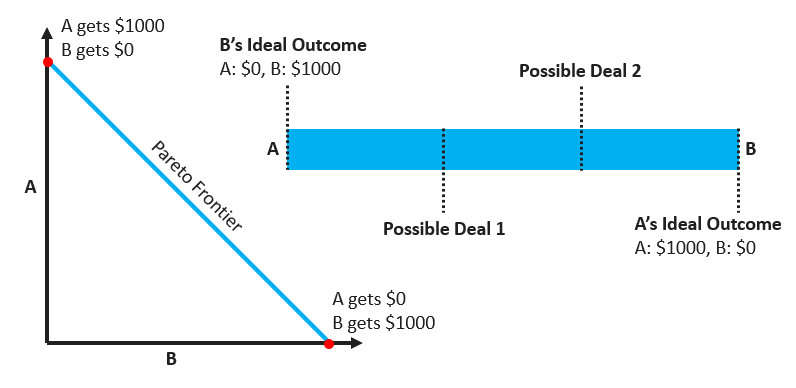
\includegraphics[width=\textwidth,height=0.9\textheight,keepaspectratio]{Bargaining.png}
\end{frame}

\begin{frame} 
 \frametitle{\LARGE{Game Theory Implications for IR}}
 	\begin{itemize}
 		\item How can we encourage better outcomes for cooperation between actors? How can actors escape the trap of the PD and collective action problems? \pause \\~\\
 		\begin{enumerate}
 			\item Number and relative size of actors \pause \\~\\
 		    \item Iteration \pause \\~\\
 		    \item Linkage \pause  \\~\\
 		    \item Information  \\~\\
 		\end{enumerate}
 	\end{itemize}
 \end{frame}

\begin{frame} 
	\frametitle{\LARGE{Number and Relative Size}}
	\begin{itemize}
		\item Easier for smaller number of actors to cooperate and monitor each other’s behavior, preventing opportunities for defection. \pause
		\item For public good provision, it may be in the interest of a relatively large member to provide the good for the group—if that member receives benefits sufficient to justify the entire costs.
		\begin{itemize}
			\item Ex: National defense; US funding NATO
		\end{itemize}
	\end{itemize}
\end{frame}

\begin{frame} 
	\frametitle{\LARGE{Iteration}}
	\begin{itemize}
		\item Cooperative outcomes are more likely when actors have repeated interactions. \pause
		\item Why? Even if defection incentives exist in current interaction, if other actors withhold their cooperation in the future in interactions with “defectors”, actors may be induced to cooperate by fear of losing future benefits.
		\begin{itemize}
			\item Ex: Iterated Prisoner's Dilemma sees actors converge on cooperation.
		\end{itemize}
	\end{itemize}
\end{frame}

\begin{frame} 
	\frametitle{\LARGE{Issue Linkage}}
	\begin{itemize}
		\item \textbf{Issue Linkage}: Tying cooperation in one policy area with cooperation in another area.		
		\item ``I'll cooperate here if you cooperate there." \pause
		\item Differs from iteration as iteration focuses on the future, while this focuses on other policy areas in the present.
	\end{itemize}
\end{frame}

\begin{frame} 
	\frametitle{\LARGE{Information}}
	\begin{itemize}
		\item Providing information allows actors to coordinate their responses. \pause
		\item Imagine the Prisoner's Dilemma, but both prisoners are in the same cell and can communicate...
	\end{itemize}
\end{frame}

\begin{frame} 
	\frametitle{\LARGE{Institutions and Anarchy Redux}}	
	\begin{itemize}
		\item Recall the puzzle from earlier in class: Despite anarchy, most states follow institutional rules most of the time. Why? \pause
		\item \textbf{Institutions enable cooperation by providing information, creating iteration, and enabling issue linkage.} \pause
		\item In this way, institutions can facilitate cooperation that would have been unlikely without them. \pause
		\item It is less costly to use existing institutions, even if imperfect, than to establish new ones.	
	\end{itemize}
\end{frame}

\begin{frame} 
	\frametitle{\LARGE{Institutions and Anarchy Redux}}	
	How do institutions accomplish this? \pause
	\begin{itemize}
		\item Setting standards of behavior
		\item Verifying compliance with rules and decisions
		\item Reducing the costs of joint decision making
		\item Selecting rules of interaction that make cooperation more likely	
	\end{itemize}
	Even biased institutions can still be helpful in this regard.
\end{frame}

\begin{frame} 
	\frametitle{\LARGE{Institutions and Policy Bias}}	
	\centering
	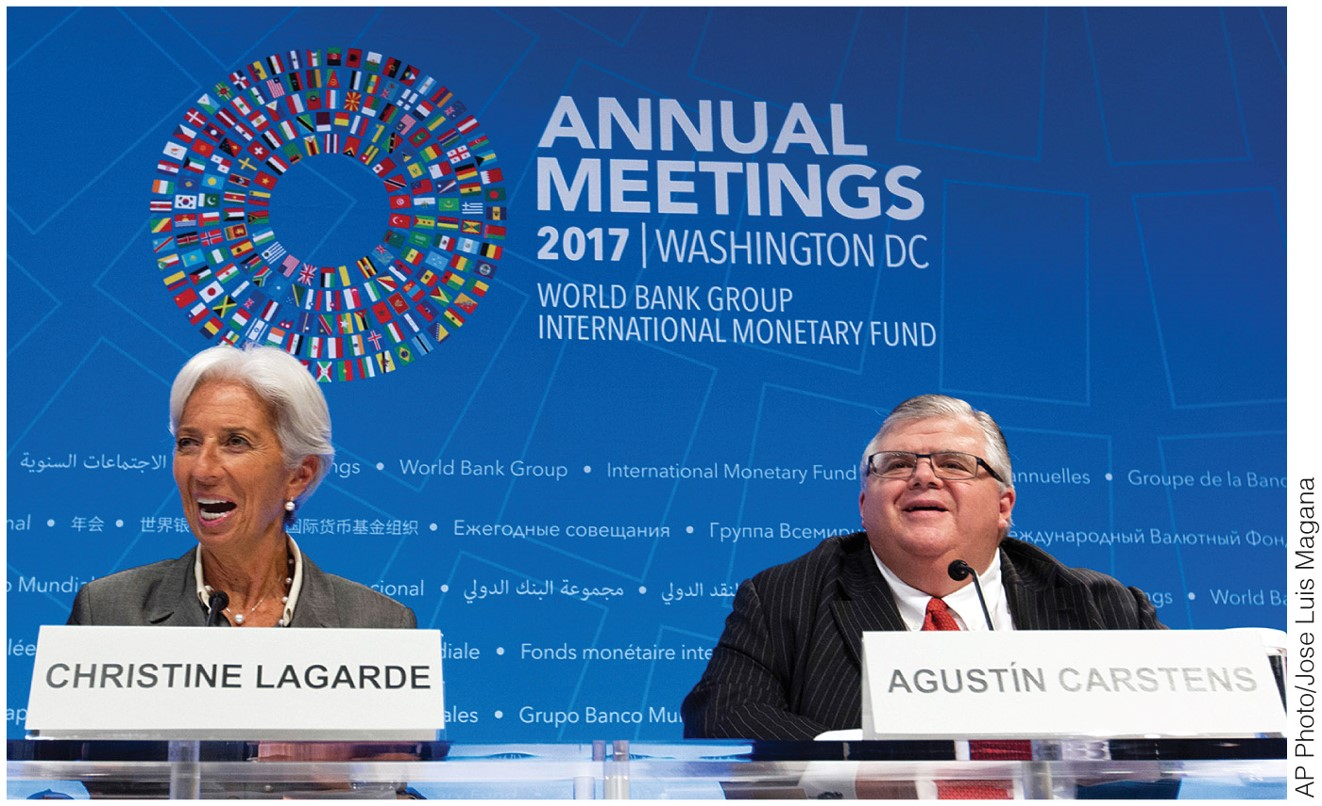
\includegraphics[width=\textwidth,height=0.9\textheight,keepaspectratio]{IMF2017.jpg}
\end{frame}

\begin{frame} 
	\frametitle{\LARGE{Institutional Bias}}	

	\begin{itemize}
		\item Example: the International Monetary Fund (IMF).
		\item The EU and the US each have enough votes within the IMF to veto any major decision by the organization. \pause
		\item Many critics charge that the IMF, as a result, is biased in its policies toward the interests of the developed countries. \pause
		\item Few (no?) institutions are wholly neutral.
	\end{itemize}

\end{frame}

\begin{frame} 
\frametitle{\LARGE{Summary}}
    \begin{itemize}
    	\item To develop theories of political behavior, we identify actors, their interests, how they interact, and how institutions structure those interactions. \pause
    	\item Most interactions are strategic interactions. \pause
    	\item We can analyze strategic interactions through game theory. \pause
    	\item Game theory requires that we assume actors are rational. \pause
    	\item This assumption yields interesting results: cooperation and bargaining in general, as well as the PD and collective action problems. \pause
    	\item International institutions can enable beneficial cooperative outcomes even in an environment of anarchy.         
    \end{itemize}
\end{frame}

\end{document}
